\chapter{Shapes as Metric Spaces}
\label{chapter:shapeSpaces}
%some stuff about normal distances.
The main question this chapter will be answering is, whether or not there exists such a thing as a ``space of shapes'' and if so, how to discern shapes from each other.
To achieve this, we need the notion of a distance on a shape, in other words, we have to define a metric.

\section{Metrics}
%%%%%%%%%%%%%%%%%%%%%%%%%%%%%%%%%%%%%%%
%%
%%      Metrics
%%
%%%%%%%%%%%%%%%%%%%%%%%%%%%%%%%%%%%%%%%
We start by defining the most important point of this section, the metric space.
\begin{mydef}[metric space]
	A set $M$ is called a metric space, if for each pair of points $x,y \in M$ there is a distance/metric function $d_M: M \times M \rightarrow \real_+ \cup \{0,\infty\}$ such that:
	\begin{itemize}
		\item $d_M(x,y) = 0 \Leftrightarrow x = y$ (identity of indiscernibles)
		\item $d_M(x,y) = d_M(y,x)$ (symmetry)
		\item $d_M(x,y) \le d_M(x,z) + d_M(z,y)\,\forall x,y,z \in M$ (triangle inequality)
	\end{itemize}
\end{mydef}
In other words, if we can find a distance function which fulfills the given properties, every set can be a metric space.
The ones most important to this thesis are the metric spaces defined on all three dimensional shapes.
But what are the interesting properties of such a metric space?
For one, there then exists a way to measure how ``close'' one shape is to another by watching its individual points and comparing the behavior of the metric function over the shapes.
One interesting term in this context is the isometry:
\begin{mydef}
	A surjective, distance-preserving map $f$ is called an isometry, where $f$ being distance preserving means that for $f :X \rightarrow Y$ the equation $d_X(x,y) = d_Y(f(x),f(y)) \,\forall x,y \in X$ holds.
	Two metric spaces $(X,d_X)$ and $(Y,d_Y)$ are isometric, if there exists such an isometry $f :X \rightarrow Y$.
\end{mydef}
Thus, if a shape undergoes a isometric transformation, the distance retained.
The more intuitive way of describing isometries is, that there are two instances of the same shape and one is changed a little, like for example by being rotated or scaled.
There is also the notion of near-isometries for almost isometric shapes, like a human in two different poses (which are not isometric, since there is some bending and stretching of the surface).

Another thing, we are assuming from here on is that our metric spaces are compact.
A metric space being compact implies that it is closed/complete and totally bounded, which is a reasonable call, since the surfaces we are interested in can mostly be approximated by 3D-meshes.
\begin{mydef}[sequentially compact]
	A subset $X \subset Y$ of a metric space $Y$ is sequentially compact if every sequence in $X$ has a convergent subsequence whose limit belongs to $X$.
	Explicitly this means that for each sequence $(x_n)$ with $x_n \in X$, there exists a subsequence $(x_{n_k})$ such that for $k \rightarrow \infty$ the subsequence$(x_{n_k}) \rightarrow x$ converges to a point $x\in X$.
\end{mydef}

Now there are a few interesting properties of metric spaces.
If $(X,d_X)$ is a metric space and $Y \subset X$, then a metric function for $Y$ can be obtained by the restriction of $d_X$ to the subset $d_Y = \left.d_X\right|_Y$.
This is a useful property because, for example if we wish to compare a part of a surface to the whole, the metric is unchanged on the partial surface.
Moreover, $X$ is called ambient space for $Y$ and even though the restriction of $d_X$ is the simplest, it is not the only way to define a metric on $Y$.
In many cases, there is a more natural intrinsic metric, which means that it is not dependent on the ambient space.
Now, to define the distance of a point $x \in X$ to a subset $Y$, the smallest distance between $x$ and $Y$ is used: $d_X(x,Y) = \inf_{y \in Y} d_X(x,y)$.

\begin{example}
Let us consider the metric space $(\real^2, \|\cdot\|)$ with the euclidean metric and its subset $S \subset \real^2$ containing the points of the unit circle.
The restriction of $\|\cdot\|$ to $S$ would be a possible metric function, but a more intuitive, intrinsic metric is the minimal arc length between two points.
It is easily to be seen, that the minimal arc length is in fact a metric, since it is symmetric, equal to zero if the points are equal and there is no shorter way over a third point and so the triangle inequality is also fulfilled.
Additionally the arc length does not depend on the $\real^2$ coordinates of the points but on their position on the unit circle, what makes the minimal arc length an intrinsic metric.
The two proposed metrics are also not isometric, as the distance between two opposing points $x,y\in S$ is different: $\|x,y\| = 1$ while $minarclength(x,y) = 2\pi$.
\end{example}
%compactness -> diam < inf
% ?:diameter of S, distance of point and set

So if we can define some sort of distance function between shapes, we could distinguish between shapes with small differences (e.g. two humans in different positions) and shapes with big differences like a human and a car.

\section{Gromov-Hausdorff distance}
%%%%%%%%%%%%%%%%%%%%%%%%%%%%%%%%%%%%%%%
%%
%%      Gromov-Hausdorff
%%
%%%%%%%%%%%%%%%%%%%%%%%%%%%%%%%%%%%%%%%
The most commonly used metric to differentiate three dimensional shapes is the Gromov-Hausdorff distance.
But before we begin working on the Gromov-Hausdorff distance, we need to find a intuition of what it means for surfaces to be ``close'' to each other.
Smooth surfaces in $\real^3$ can (at least locally) be parametrized by a domain $U \subset \real^2$ for example by an embedding $f: U\rightarrow \real^3$.
%TODO? picture: surface <- f1 - U - f2-> surface2
Two parametrizations then specify a homeomorphism from one surface to the other.
Those two surfaces are said to be ``close'' if the homeomorphism only slightly changes some properties, like distances or derivatives, of the surfaces.

To start off, we consider the problem of comparing two shapes in the same metric space.
For that the Hausdorff distance as seen in figure~\ref{fig:hausdorff} is used.
\begin{mydef}[Hausdorff distance]
	The Hausdorff distance between two compact subsets $X,Y \subset (Z,d_Z)$ is defined by
	$$d^Z_\mathcal{H}(X,Y) = \max \left\{ \sup_{x \in X} d_Z(x,Y), \sup_{y \in Y} d_Z(y,X)\right\}.$$
	$d^Z_\mathcal{H}(X,Y)$ is a semi-metric on the space of compact subsets of a metric space.
\end{mydef}
Even though it is called distance, the Hausdorff distance is only a semi-metric since there are cases, where $d^Z_\mathcal{H}(X,Y) = 0 \Leftrightarrow X = Y$ does not hold.
Take for example the set $X = (0,1)$ and its closure $Y = [0,1]$.
So the biggest distance should be between either $0$ or $1$ and $X$ which in both cases is zero although $X \neq Y$.
Also note, that even one stray point can make the Hausdorff distance arbitrarily large.

\begin{figure}[h]
	\centering
	\includegraphics[width = 0.5\textwidth]{pictures/hausdorff}
	\caption{A visualisation of the two relevant distances of the Hausdorff distance: $d_1 = \sup_{x \in X} d_Z(x,Y)$ while $d_2 = \sup_{y \in Y} d_Z(y,X)$. The Hausdorff distance is defined as the bigger one, $d_2$ in this case.}
	\label{fig:hausdorff}
\end{figure}

But with the Hausdorff distance, we can only find the distance between sets which are subsets of a common metric space.
To be able to define a distance between different metric spaces $X,Y$, the basic idea is to use a isometric embedding into another metric space $Z$ and use the Hausdorff-distance there.
The Gromov-Hausdorff distance $d_\mathcal{GH}(X,Y)$ is defined as the minimum $r$ for which such an embedding space $Z$ and the isometric embeddings $X',Y'\subset Z$ exist with $d^Z_\mathcal{H}(X,Y) < r$.
\begin{mydef}[Gromov-Hausdorff]
	The Gromov-Hausdorff distance between two metric spaces $X$ and $Y$ is defined by
	$$d_\mathcal{GH}(X,Y) = \inf_{Z,f,g} d^Z_\mathcal{H}((f(X), g(Y))$$
	taken over all ambient spaces $Z$ and isometric embeddings $f:X \rightarrow Z, g: Y \rightarrow Z$.
\end{mydef}
$d_\mathcal{GH}(X,Y)$ is a metric on the space of isometry classes of compact metric spaces thus we can say that there exists a ``space of shapes''.
Note however, that from a practical perspective, the possibilities for choosing $Z,f$ and $g$ are far to huge to simply compute the Gromov-Hausdorff distance directly without further restrictions.

To begin with, we restrict the search space to possible correspondences between $x$ and $Y$.
\begin{mydef}[correspondence]
	A correspondence between two sets $X$ and $Y$ is a set $R \subset X \times Y$ which satisfies
	\begin{itemize}
		\item for all $x \in X$ there exists $y\in Y$ such that $(x,y) \in R$.
		\item for all $y \in Y$ there exists $x\in X$ such that $(x,y) \in R$.
	\end{itemize}
\end{mydef}
Note that a correspondence neither has to map one point to exactly one other nor does every point have to be a part of the correspondence.
A correspondence $R$ is associated to a map $f: X \rightarrow Y$ if $R = \{(x,f(x)) :x \in X\}$ contains the image of $f$.
Our next target is to show that the Gromov-Hausdorff distance can be alternatively defined by using correspondences between two metric spaces.
Remember that the Gromov-Hausdorff distance was defined to measure the difference between two metric spaces.
\begin{figure}[h]
	\centering
	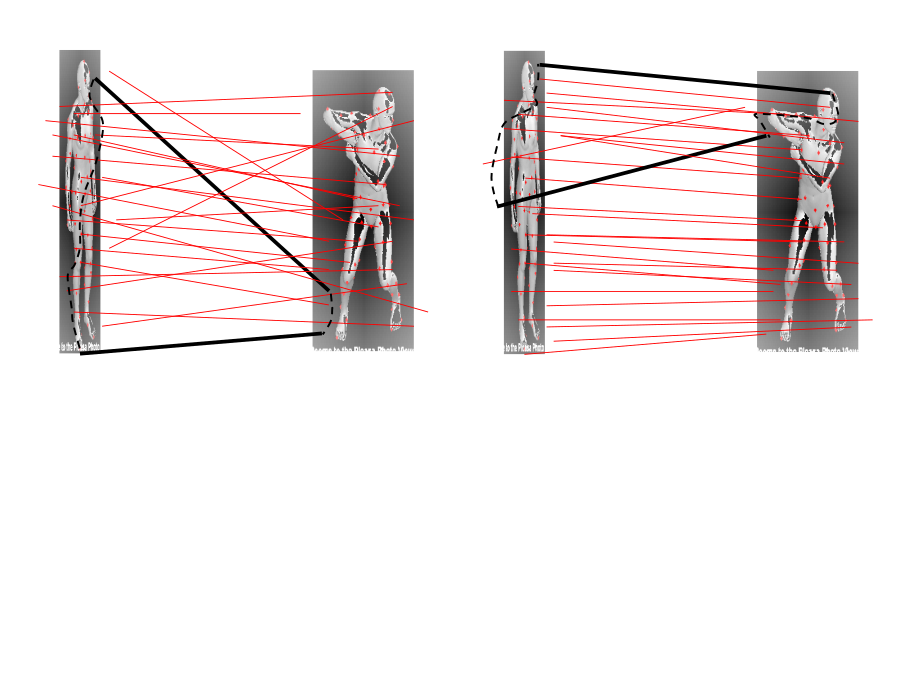
\includegraphics[width = 0.9\textwidth]{pictures/metric_distortion}
	\caption{The figure shows two different given correspondences.
		For the black correspondences, additionally the shortest path between them is given.
		Since the metric distortion measures the change of these distances by the correspondence, we can see that the distance on the left shape is not being preserved, while the distance on the right set of meshes is preserved almost perfectly.
		Therefore the correspondence on the left side results in great metric distortion, whereas the right correspondence will have a lower distortion, based on the given distances.}
	\label{fig:metric_distortion}
\end{figure}
Now we can define the distortion between two given metric spaces by using a correspondence.
\begin{mydef}[metric distortion]
	Let $(X,d_X)$ and $(Y,d_Y)$ be compact metric spaces and $R \subset (X,d_X) \times (Y,d_Y)$ be a correspondence.
	Then the distortion of $R$ is defined as
	\begin{equation}
		dis\,R = \sup\{\,|d_X(x,x') - d_Y(y,y')|: \left( (x,y), (x',y') \in R \right)\}.
	\end{equation}
\end{mydef}
How the distortion of a metric shows on meshes can be seen in figure~\ref{fig:metric_distortion}.
By the definition of isometry, the distortion of $R$ is zero if and only if the map associated with $R$ is an isometry.
This leads to another definition of the Gromov-Hausdorff distance.
\begin{mydef}[Gromov-Hausdorff distance (2)]
	The Gromov-Hausdorff distance between two metric spaces $X$ and $Y$ is defined by
	\begin{equation}
		d_\mathcal{GH}(X,Y) = \frac{1}{2} \inf_{R \subset X \times Y} dis \, R.
		\label{eq:gromov_hausdorff}
	\end{equation}
\end{mydef}
In this formulation, the Gromov-Hausdorff distance is defined as the infimum of $r > 0$ for which there is a correspondence with $dis\,R = 2r$.
And unlike the first definition, we now minimize over a finite set of correspondences instead of all possible ambient spaces and their corresponding embeddings.
% coverings, fps

Another improvement is to use open ball coverings of the metric spaces.
This means that instead of using all points within a metric space, we choose representatives such that they cover all points on the mesh.
\begin{mydef}[open ball covering]
	Let $x \in (X,d_X)$ be a metric space. An open ball of radius $r > 0$ centered at x is defined by
	$$B_X(x,r) = \{z\in X:d_X(x,z) < r\}.$$
	For a subset $A \subset X$, we define the open ball as
	$$B_X(A,r) = \bigcup{a\in A} B_X(a,r).$$
	A set $C\subset X$ is a r-covering of $X$ if $B_X(C,r) = X$.
\end{mydef}
The interesting point of this is that the r-covering of a shape is close to the original shape in a Gromov-Hausdorff sense.
Let $\{x_1,\ldots,x_n\}\subset X$ be a r-covering of a compact metric space $(X,d_X)$.
Then $d_\mathcal{GH}(X,\{x_1,\cdots,x_n\}) \le r$ holds as stated in \cite{burago2001course}, which means that $d_\mathcal{GH}$ is consistent to sampling.
This further leads to us only having to compute $d_\mathcal{GH}$ for a dense enough r-covering of our metric spaces $X$ and $Y$ to have a good approximation of its behavior in the originally continuous spaces.
Also, this shows that the approximation of shapes by triangulated meshes, which more or less are point samples, is well posed in this context up to a certain error.

Since it is not easy to compute an optimal covering, the farthest point sampling was devised.
It is efficient to compute, once the metric function is available and is at most worse than an optimal sampling by a factor of two.
Its basic idea is to iteratively select points from the metric space, until the needed number of points is reached.
The algorithm is initialized by either choosing a arbitrary point or by choosing two points which are the farthest away from each other and declaring them as our initial covering $C_0$.
After that, the algorithm selects a point $x$ fulfilling the equation $\underset{x}{\operatorname{arg\,max}} d_X(x,C)$ in each step, adding it to the previously selected $C_k = C_{k-1} \cup \{x\}$.
The result is a progressively denser sampling of the shape which in general is not unique but ``almost'' optimal.
This can then be used to create a Voronoi sampling of the shape by assigning all points to their closest sampled point $x \in C_k$.
%TODO again citecitecite, perhaps a more beautiful ending

%minimising the gromov-hausdorff distance is a common approach followed in shape analysis.
%this leads to a relaxed quadratic assignment problem
%figures: meshes matched this way
Minimizing the Gromov-Hausdorff distance is a common approach followed in shape analysis.
In order to reduce the problems complexity, the equation from \eqref{eq:gromov_hausdorff} can be relaxed to a quadratic assignment problem \cite{memoli2007use}, for which there exist a number of optimization algorithms.
